\subsection{\emph{Contiki}}

\subsubsection{Installation}

\emph{Contiki} se présente sous la forme d’une machine virtuelle \emph{Ubuntu} où sont préinstallées les paquets ou les sources de divers logiciels utiles au développement d’application pour des cartes électroniques.

La VM se trouve sur le site de \emph{Contiki} (\url{http://www.contiki-os.org/download.html}), une fois télécharger, on se retrouve avec une VM au format \emph{VMWare}, ce qui fait quelle n'est pas compatible avec \emph{VirtualBox}.
Si on veut vraiment travailler avec \emph{VirtualBox} alors \emph{VMWare} propose un outil de conversion qui permet de convertir la VM dans une format open-source, le \texttt{ova}.

Il faut donc installer les deux outils puis dans un terminal (ou une invite de commande) entrer :
\begin{verbatim}
./ovftool [original .vmx location and filename]
	[new .ova location and filename]
\end{verbatim}
Ce qui peut donner sous un Linux :
\begin{verbatim}
./ovftool ~/Download/contiki.vmx ~/Download/contiki.ova
\end{verbatim}

Une fois l'opération terminé on peut alors importer la VM sur \emph{VirtualBox} qui fonctionnera exactement de la même manière que sur \emph{VMWare}.
 
\subsubsection{Cooja}

\emph{Contiki} inclue un logiciel pour la simulation de communications entre plusieurs objets connectés, \emph{Cooja}.

En suivant le tutoriel de prise en main \citeweb{getting-started}, nous avons commencé notre utilisation de \emph{Contiki} en testant l’exécution d’un des programmes donnés en exemple.
\emph{Cooja} n’étant pas livré avec un émulateur pour la CC 2538, nous avons utilisé une simulation d’une « \textit{Sky mote} ».

\begin{figure}[H]
\centering
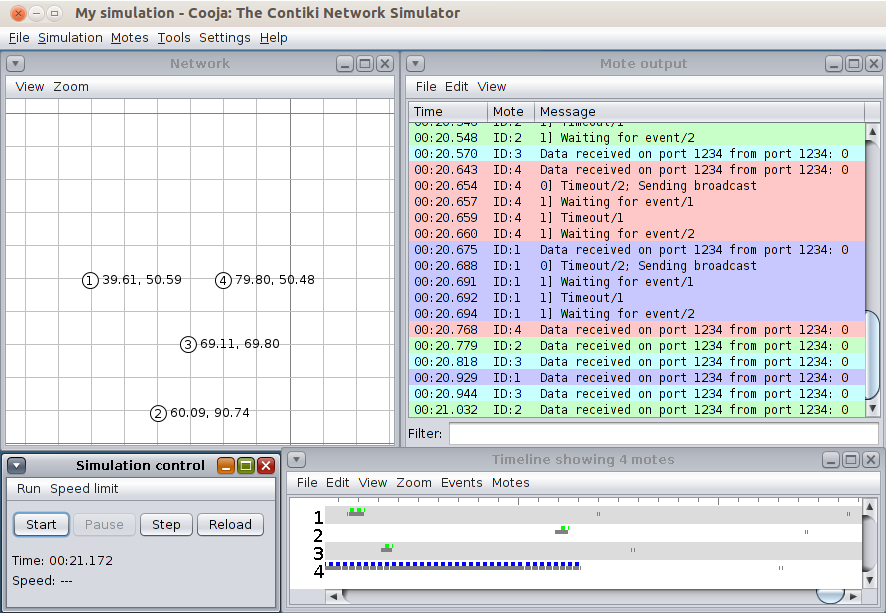
\includegraphics[width=15cm]{\rpDossier/images/cooja.PNG}
\caption{Simulation avec Cooja}
\label{cooja}
\end{figure}

\emph{Cooja} est conçu pour pouvoir définir de nouveaux émulateurs.
Une recherche sur Internet nous a permis de découvrir que d’autres personnes ayant souhaité un tel émulateur avaient été invitées à l’écrire elles-même, sans que nous ayons pu trouver le résultat — si le conseil a été suivi.
Comme l’utilisation du simulateur n’était pas primordiale dans notre projet, nous avons donc décidé de nous concentrer sur le développement directement sur les cartes.

\subsubsection{Architecture des programmes}

Les programmes compilés avec \emph{Contiki} sont constitué d’un unique exécutable qui sera installé dans la mémoire de la carte cible.
Afin de faciliter le développement modulaire, les bibliothèques de \emph{Contiki} incluent un mécanisme de processus légers à ordonnancement coopératif \citeweb{processes}.

\paragraph{Processus}

Nous n’avions initialement pas connaissance de l’implémentation exacte des ces processus légers, ce qui a été à l’origine de dysfonctionnements dont nous avons mis du temps à trouver la cause.
Le mécanisme utilisé, conçu pour économiser la mémoire, implique en effet des contraintes de programmation auxquelles nous n’étions pas habitués :
\begin{itemize}
	\item la valeur des variables locales peut changer lors de l’appel à une des macros de contrôle des procesus ;
	\item certaines portions du code peuvent être exécutée à des moments inattendus.
\end{itemize}

En effet, les processus sont implémentés sous forme de \emph{protothreads}, c’est-à-dire de \emph{threads} sans sauvegarde de la pile \citeweb{protothreads}.
Chaque processus est une procédure (en pratique un pointeur de fonction) qui est appelée à chaque fois que le processus est activé.
Les processus rendent la main à l’ordonnanceur lorsque cette procédure se termine (instruction \texttt{return}).

Les macros fournies par \emph{Contiki} permettent de sauvegarder la position du code en cours d’exécution et d’y retourner en donnant l’impression de fonctionner comme une bibliothèque de \emph{threads} (par exemple en fournissant des pseudo-instructions \texttt{PROCESS\_YIELD} et \texttt{PROCESS\_WAIT\_EVENT}).
La pile est cependant utilisée par d’autres processus entre la mise en pause du processus et son réveil, modifiant l’état des variables locales non statiques.
Avant d’avoir compris ce mécanisme, nous avons utilisé une variable de boucle dont le comportement étrange de la valeur nous a poussé à faire l’étude précise de ce fonctionnement.
\label{variables-locales}

D’autre part, le code situé avant la macro \texttt{PROCESS\_BEGIN} est exécuté à chaque réveil du processus.
Nous n’avons pas eu de problème avec ce comportement, l’ayant compris avant de tenter des modification dans cette zone.
En revanche, sa connaissance nous a été utile pour comprendre des blocages que nous avons eu avec les \emph{timers}, en y plaçant du code de journalisation.

\paragraph{\emph{Timers}}

Un des processus fournis par \emph{Contiki} permet de manipuler le temps simplement : \emph{etimer} \citeweb{etimer}.
Les autres processus peuvent enregistrer un \emph{timer} auprès de ce processus, qui est en charge d’émettre un événement lorsque celui-ci arrive à expiration.

La macro \texttt{PROCESS\_WAIT\_EVENT\_UNTIL} permet d’attendre simplement l’événement émis à la fin du temps demandé, mais son utilisation dans les exemples (ajoutée à notre mauvaise compréhension des processus) nous a induits en erreur.
En effet, les exemples ne vérifient pas que l’événement reçu par le processus est bien celui qui était attendu.
Dans le contexte des exemples qui sont donnés, assez simples, ça n’a pas d’importance, mais nous avons eu par la suite des situations où deux \emph{timers} pouvaient arriver à terme presqu’au même moment dans une boucle.
Lorsque cela arrivait, si le processus de gestion des \emph{timers} les traite dans le mauvaise ordre, notre processus entrait dans une attente infinie d’un \emph{timer} dont il avait déjà reçu l’événement.

\todo[schéma du problème + clarifier la description]
